%% abtex2-modelo-trabalho-academico.tex, v-1.7.1 laurocesar
%% Copyright 2012-2013 by abnTeX2 group at http://abntex2.googlecode.com/ 
%%
%% This work may be distributed and/or modified under the
%% conditions of the LaTeX Project Public License, either version 1.3
%% of this license or (at your option) any later version.
%% The latest version of this license is in
%%   http://www.latex-project.org/lppl.txt
%% and version 1.3 or later is part of all distributions of LaTeX
%% version 2005/12/01 or later.
%%
%% This work has the LPPL maintenance status `maintained'.
%% 
%% The Current Maintainer of this work is the abnTeX2 team, led
%% by Lauro César Araujo. Further information are available on 
%% http://abntex2.googlecode.com/
%%
%% This work consists of the files abntex2-modelo-trabalho-academico.tex,
%% abntex2-modelo-include-comandos and abntex2-modelo-references.bib
%%

% ------------------------------------------------------------------------
% ------------------------------------------------------------------------
% abnTeX2: Modelo de Trabalho Academico (tese de doutorado, dissertacao de
% mestrado e trabalhos monograficos em geral) em conformidade com 
% ABNT NBR 14724:2011: Informacao e documentacao - Trabalhos academicos -
% Apresentacao
% ------------------------------------------------------------------------
% ------------------------------------------------------------------------

\documentclass[
	% -- opções da classe memoir --
	12pt,				% tamanho da fonte
	openright,			% capítulos começam em pág ímpar (insere página vazia caso preciso)
	twoside,			% para impressão em verso e anverso. Oposto a oneside
	a4paper,			% tamanho do papel. 
	% -- opções da classe abntex2 --
	%chapter=TITLE,		% títulos de capítulos convertidos em letras maiúsculas
	%section=TITLE,		% títulos de seções convertidos em letras maiúsculas
	%subsection=TITLE,	% títulos de subseções convertidos em letras maiúsculas
	%subsubsection=TITLE,% títulos de subsubseções convertidos em letras maiúsculas
	% -- opções do pacote babel --
	english,			% idioma adicional para hifenização
	french,				% idioma adicional para hifenização
	spanish,			% idioma adicional para hifenização
	brazil,				% o último idioma é o principal do documento
	]{abntex2}


% ---
% PACOTES
% ---

% ---
% Pacotes fundamentais 
% ---
\usepackage{cmap}				% Mapear caracteres especiais no PDF
\usepackage{lmodern}			% Usa a fonte Latin Modern			
\usepackage[T1]{fontenc}		% Selecao de codigos de fonte.
\usepackage[utf8]{inputenc}		% Codificacao do documento (conversão automática dos acentos)
\usepackage{lastpage}			% Usado pela Ficha catalográfica
\usepackage{indentfirst}		% Indenta o primeiro parágrafo de cada seção.
\usepackage{color}				% Controle das cores
\usepackage{graphicx}			% Inclusão de gráficos
% ---
\usepackage{comment}		
% ---
% Pacotes adicionais, usados apenas no âmbito do Modelo Canônico do abnteX2
% ---
\usepackage{lipsum}				% para geração de dummy text
% ---

% ---
% Pacotes de citações
% ---
\usepackage[brazilian,hyperpageref]{backref}	 % Paginas com as citações na bibl
\usepackage[alf]{abntex2cite}	% Citações padrão ABNT

\usepackage[brazil]{babel}



% --- 
% CONFIGURAÇÕES DE PACOTES
% --- 

% ---
% Configurações do pacote backref
% Usado sem a opção hyperpageref de backref
\renewcommand{\backrefpagesname}{Citado na(s) página(s):~}
% Texto padrão antes do número das páginas
\renewcommand{\backref}{}
% Define os textos da citação
\renewcommand*{\backrefalt}[4]{
	\ifcase #1 %
		Nenhuma citação no texto.%
	\or
		Citado na página #2.%
	\else
		Citado #1 vezes nas páginas #2.%
	\fi}%
% ---


% ---
% Informações de dados para CAPA e FOLHA DE ROSTO
% ---
\titulo{Uso de Padrões de Projetos no desenvolvimento de aplicativos Android}
\autor{Diego Lins de Freitas}
\local{Manaus-Am}
\data{2013, v0.6}
%\orientador{Lauro César Araujo}
\instituicao{%
  Faculdade Fucapi
  \par
  Especialização em Engenharia de Software
  \par
  Centro de Pós-Graduação e Extensão (CPGE)}
\tipotrabalho{Tese (Doutorado)}
% O preambulo deve conter o tipo do trabalho, o objetivo, 
% o nome da instituição e a área de concentração 
\preambulo{}
% ---


% ---
% Configurações de aparência do PDF final

% alterando o aspecto da cor azul
\definecolor{blue}{RGB}{41,5,195}

% informações do PDF
\makeatletter
\hypersetup{
     	%pagebackref=true,
		pdftitle={\@title}, 
		pdfauthor={\@author},
    	pdfsubject={\imprimirpreambulo},
	    pdfcreator={LaTeX with abnTeX2},
		pdfkeywords={abnt}{latex}{abntex}{abntex2}{trabalho acadêmico}, 
		colorlinks=true,       		% false: boxed links; true: colored links
    	linkcolor=blue,          	% color of internal links
    	citecolor=blue,        		% color of links to bibliography
    	filecolor=magenta,      		% color of file links
		urlcolor=blue,
		bookmarksdepth=4
}
\makeatother
% --- 

% --- 
% Espaçamentos entre linhas e parágrafos 
% --- 

% O tamanho do parágrafo é dado por:
\setlength{\parindent}{1.3cm}

% Controle do espaçamento entre um parágrafo e outro:
\setlength{\parskip}{0.2cm}  % tente também \onelineskip

% ---
% compila o indice
% ---
\makeindex
% ---

% ----
% Início do documento
% ----
\begin{document}

% Retira espaço extra obsoleto entre as frases.
\frenchspacing 

% ----------------------------------------------------------
% ELEMENTOS PRÉ-TEXTUAIS
% ----------------------------------------------------------
% \pretextual

% ---
% Capa
% ---
%\imprimircapa

\imprimirfolhaderosto*

% ---
% RESUMOS
% ---

% resumo em português
\begin{resumo}
 A plataforma android foi adotada por vários fornecedores de smartphones e tablet promovendo uma disseminação 
 do sistema operacional muito abrangente. Formou-se um grande mercado a ser explorado com fornecimento de 
 aplicativos para as  mais variadas finalidades. Para atender essa demanda é necessário desenvolver aplicativos 
 de qualidade e o mais rápido possível mas por se tratar de pequenos  aplicativos há pouca preocupação com a 
 arquitetura é deixada de lado. Os padrões difundidos na comunidade são focados na utilização de componentes e 
 desenvolvimento da interface. Neste artigo é apresentado alguns padrões de projetos  aplicados ao desenvolvimento 
 de aplicativos android dando um visão mais ampla de um aplicativo. 

 \vspace{\onelineskip}
    
 \noindent
 \textbf{Palavras-chaves}: Android. MVC. MVP.
\end{resumo}

% ---
% inserir o sumario
% ---
\pdfbookmark[0]{\contentsname}{toc}
\tableofcontents*
\cleardoublepage
% ---

% ----------------------------------------------------------
% ELEMENTOS TEXTUAIS
% ----------------------------------------------------------
\textual

\chapter{Introdução}

%Contextualização android vai dominar precisamso programar pra ele
A tendência do mercado de dispositivos móveis é aumentar. Segundo IDC,  é
experado um crescimento de 32.7\% na produção em 2013 \cite{idc:a}. O sistema
operacional android é o líder dominando 75\% desse mercado com mais de 162 milhões de
smartphones produzidos e embarcados com android\cite{idc:b}. Baseado nesses
dados é possível concluir que existe uma damanda no desenvolvimento de novos 
aplicativos que agregem valor à esses aparelhos.
% é preciso que tenha   - Design Principles.

Para produzir aplicativos de qualidade é necessário aplicar boas práticas de
desenvolvimento de software. Levando-se em consideração que a linguagem de
programação usada para o desenvolvimento na plataforma android é a Java, é
natural que se aplique as práticas definidas pelos princípios de projeto
orientado a objetos. Esses princípios guiam o desenvolvedor em como definir a
estrutura interna do software afetando diretamente características  de
qualidade como manutenabilidade, performance e outras\cite{tempero-di}.

Os padrões de projeto são aplicados na engenharia de software como forma de
reproduzir  soluções  para problemas recorrentes melhorando a manutenabilidade e
o reuso de componentes de software\cite{gof}.O uso de padrões de projetos
é um meio de aplicar esses princípios. 

Boas práticas de engenharia de software promevem o desenvolvimento dos
artefatos que constituem o sistema de forma coesa. Os conjuntos desses artefatos
podem ser classificados de acordo com suas responsabilidades, surgindo
uma divisão clara em camadas. Um sistema pode ter diversas camadas responsáveis
por acesso à um banco de dados, cominicação com serviços externos, encapsular
regras de negócio. Uma dessas camadas que constituem um aplicativo androia é a
camada de apresentação ou interface com o usuário.
 
Segundo \citeonline{pressman}, ``A interface com o usuário pode ser considerada
o elemento mais importante de um sistema ou produto baseado em computador``.
tendo em vista isso, será tratado nesse trabalho  os padrões para
desenvolvimento da camada de apresentação de em aplicativos android.

\section{Motivação}

A motivação para a execução desta pesquisa sugiu da participação do autor em
projetos para desenvolvimento de aplicativos android em uma instituição de
pesquisa e desenvolvimento localizada em Manaus. O comprometimento com a
qualidade promoveu o uso de ferramentas de código aberto para monitoração da
qualidade dos projetos, além do processo de testes adotado pela empresa. Com uma
equipe composta por mais de 30 desenvolvedores produzindo aplicativos com
diversas finalidades, houve a necessidades de padronização da arquitetura.

\section{Problematização}
Dado que existem uma vasta diversidade de padrões de projeto a serem aplicados
no desenvolvimento de software, Qual padrão de projeto é aplicável para o
desenvolvimento da camada de apresentação de aplicativos android para melhorar a
qualidade do produto final?

\section{Hipótese}

O padrão de projeto Model-View-Presenter é aplicável no desenvolvimento da
camada de apresentação de aplicativos android, gerando um aumento da qualidade
do produto final.

\section{Objetivos}

Este trabalho fará um estudo sobre a arquitetura de aplicativos android com o
propósito de melhorar a qualidade desses softwares, causando uma redução nos
riscos relacionados as mudanças que acontecem durante o ciclo de desenvolvimento
e promova a reutilização de componentes e que permita o incremento de funcionalidades com
baixo impacto. Este estudo fornecerá insumos para que os desenvolvedores possam
ter uma visão geral da aplicabilidade dos padrões de projetos e analisar quais
técnicas contribuem para o seus projetos. Este trabalho tem como meta:

\begin{itemize}
\item Estudar os padrões de projeto que podem ser usados para a implementação da
camada de apresentação de um aplicativo android.
\item Avaliar os componentes do  framework android, identificando seus papéis e
responsabilidades de acordo com os padrões estudados, levando  em consideração
características que podem dificultar a aplicação dos padrões. 
\item Identificar os impactos nas características de qualidade do aplicativo de acordo
com o paradigma da Orientação a objetos.
\item Elaborar um referência de implementação para a  camada de apresentação de um
aplicativo android utilizando padrões de projetos.
\end{itemize}

\section{Trabalhos Relacionados}

Na dissertação de \citeonline{turk} é feita uma análise dos impactos na
qualidade ao aplicar cinco padrões de projetos em um software de comunicação
TCP/IP. Os resultados do trabalho citado mostram que a qualidade do software
aumenta ao aplicar padrões de projetos sendo que o principal atributo de
qualidade aferida é a manutenabilidade.


\section{Contribuições}


Tendo em vista que padrões de projetos descrevem soluções genéricas, este
trabalho tem como principal contribuição uma interpretação do padrão de projeto
Model-View-Presenter, proporcionando uma referência prática aplicada ao
framework android.

A diversidade de projetos de software torna difícil inferir se as métricas
podem ser consideradas um paramêtro para determinar a qualidade. O presente
trabalho  se propõe a avaliar a aderência do padrão MVP â projetos android
através de indicadores de qualidade de código orientado a objetos.

\section{Organização do Trabalho}

Será descrito a metodologia, definicão do projeto, experimentos, conclusões.


\chapter{Metodologia}

Esta pesquisa se caracteriza como experimental pois tem fins práticos ao
realizar uma revisão na literatura existente sobre orientação a objetos e seus
princípios bem como referências sobre padrões de projetos para proporcionar o
embasamento que auxiliará na identificação dos componetes do android que podem
assumir as responsabilidades definidas nos padrões e definir como implementa-los.

Para validar a hipótese apresentada neste trabalho a pesquisa terá uma
abordagem quantitativa através da análise de dados estatistícos de métricas 
que expresssam atributos de qualidade em software orientado a objetos. O
conjunto de métricas a serem usadas nessa validação será o elaborado por
\citeonline{cksuite}.

Essas medidas serão coletadas através de um procedimento experimental em
laboratório utilizando um processo iterativo-incremental para executar
refatorações no código do objeto de estudo afim de introduzir o padrão de
projeto Model-View-Presenter e a cada iteração será feita a coleta das
métricas. Para executar esse processo será identificado um conjunto de
funcionalidades que o aplicativo atende, relacionda com a camada de
apresentação com a qual o usuário interage.

\section{Objeto de Estudo}


O projeto a ser refatorado será o aplicativo de Contatos do
android\footnote{https://github.com/android/platform_packages_apps_contacts},
que é um dos aplicativos básicos pré-instalados com o sistema operacional. Este
projeto é opensource mantido pelo  The Android Open Source Projeto suportado
pela Google com contribuições de desenvolvedores do mundo todo.

Os critérios para a escolha do objeto de estudo são:

\begin{enumerate}
  \item Tamanho/Complexidade - Um projeto muito complexo iria inviabilizar a
  pesquisa devido ao esforço para fazer a refatoração. Métricas coletadas
  apartir de projetos simples e triviais não forneceriam dados suficientes para
  uma análise satisfatória.
  \item Código Aberto - Além de permitir o acesso ao código fonte sem
  limitações para a pesquisa, tem a contribuição de vários desenvolvedores com
  experiência e formação em programação diversificada que se refletem no código fonte.
  \item Origem do projeto - A escolha de um aplicativo mantido sobre o mesmo
  gerenciamento que o sistema operacional android foi feita com o intuito de
  fazer a pesquisa em um código fonte que expressasse as técnicas e práticas de
  programação difundidas nesse ecossistema.
\end{enumerate}

\section{Processo de Experimentos}


A Figura \ref{processo_experimentacao} demonstra as atividades do processo de
experimentação adotado:
\begin{figure}[!h]
	\centering
	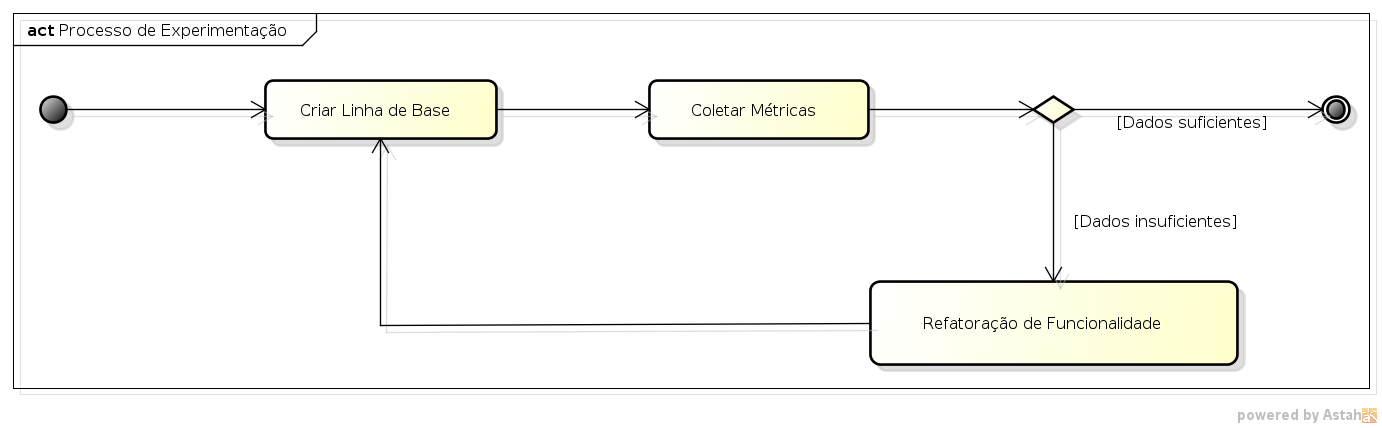
\includegraphics[scale=0.5]{img/processo_experimentacao.png}
	\caption{Processo de Experimentação Fonte: Próprio Autor}
	\label{processo_experimentacao}
\end{figure}

\begin{description}
\item[Criação uma linha de base] - Delimitar um marco do estado do código no
repositório.
\item[Refatoração Incremental] Esta atividade tem como objetivo aplicar os
padrões propostos em uma funcionalidade do aplicativo.
\item[Coleta de Métricas] Este passo tem como objetivo fazer a coleta
das métricas do código que se encontra no repositório a partir de uma revisão
para fazer a avaliação dos efeitos da refatoração na qualidade do código.
\end{description}

Esta pesquisa se propõe a executar três iterações.


\chapter{Referencial Teórico}

\section{Princípios e Padrões de Projetos}

%como referências sobre padrões de projetos para proporcionar o que auxiliará na
%identificação dos componetes do android que podem assumir as responsabilidades
%definidas nos padrões e definir como implementa-los.


Desenvolver software orientado a objetos é um desafio. Criar uma representação
computacional de uma faceta da realidade em que seus constituintes trabalhem de
forma harmoniosa para atingir as necessidades que o software se propõe a
atender requer experiência, conhecimento do domínio do problema e um processo de
análise e projeto. Apesar de existir várias abordagens para se conceber um
sistema orientado a objetos\cite{evans2004ddd},\cite{gomma11} um sistema bem
contruído apreseta características fundamentais como alta coesão e
baixo acoplamento 

designReusableClasses

Um padrão, dentro do contexto de estudo deste trabalho pode ser definido
como uma técnica efetiva cuja a sua aplicabilidade é aceita e difundiida dentro
de uma área de conhecimento com a intenção de atingir um
objetivo\cite{MetskerWake06}.

Em desenvolvimento de software, o catálogo mais difundido de padrões de projetos
orientado a objetos é elaborado por \citeonline{gof}, contendo um total de 23
padrões formalmente documentados que acumulam experiências bem sucedidas em
diversos sistemas. Esses padrões têm a seguinte classificação:

\begin{description}
\item[Criacionais] Padrões que definem como criar novas instâncias de classes.
\item[Estruturais] Foca na estruturação das classes e objetos.
\item[Comportamentais] Definem como as classes e objetos interagem entre si e
suas responsabilidades.
\end{description}

%argumentação
Analisando a forma como um padrão de projeto é concebido, com uma definição
dos papéis de cada elemento participante e como eles interagem entre si,
pode-se concluir que o uso dos padrões de projeto promove maior coesão, melhor
separação de interesses e baixo acoplamento no sistema. Todas essas
características são muito importantes e contribuem para um software de melhor
qualidade.


%Melhorar isso

%Linkar com as metricas, mostrar relação metricas e padroes

\section{Métricas de qualidade OO}
\label{sec:metrics}

Com o advento de novas técnicas de desenvolvimento de software é necessário
obter informações do impacto dessas inovações nos resultados de um projeto. Com
esse objetivo \citeonline{cksuite} elaboram um conjunto de métricas para
mensurar a qualidade de sistemas desenvolvido usando o paradigma orientado a objetos que
não se limitasse a uma linguagem de programação, fácil de coletar e com forte
embasamento teórico na ontologia de bunge\footnote{}. This model is used to analyze
some static and dynamic properties of an information system and to examine the
question of what constitutes a good decomposition of an information
system\cite{WandWeber}As métricas são:

%Bunge’s ontology has
%considerable appeal for 00 researchers since it deals with the
%meaning and definition of representations of the world, which
%are precisely the goals of the object oriented approach [32]



\begin{description}
\item[Acoplamento entre objetos (CBO)] Número de classes que ela depende por
meio da relação de composição. Uma classe está acoplada a outra quando o método
de um classe invoca o método de uma variável de instância de outra classe que
gera uma dependência entre essas classes. Quanto maior essa dependência, mais
difícil é reutilizar esses componetes em outras partes do sistema, além do
aumento do risco de efeitos colaterais ocorrerem ao modificar uma classe
altamente acoplada.
\item[Ausência de coesão dos métodos(LCOM)] Usado para avaliar a coesão de uma
classe através da similaridade entre seus métodos. Um método tem similaridade
com outro quando a intercessão entre os conjuntos de atributos usados por ambos
os métodos tem cardinalidade maior que zero. LCOM mostra esses conjuntos nulos
indicando os métodos que usam esses atributos deveriam ser implementados em
outra classe. Essa similaridade expressa a coesão da classe.
\item[Profundidade na árvore de herança (DIT)] Nível de uma classe na
hierárquia de herança. Reflete o número máximo de elementos pai dentro da aŕvove
de classes até a raiz, o que aumenta a complexidade conforme a quantidade de
elementos envolvidos se eleva, diminuindo a previsibilidade do comportamento da
classe com vários métodos e atributos sendo herdados, principalmente com o uso
de sobrecarga de métodos.
\item[Métodos por Classe (WMC)] Serve para expressar o nível de complexidade de
uma classe basseado no número de métodos que ela possui. Isso afeta o esforço de
manutenção da classe, além de impactar nas classe filhas que herdarão esses
métodos e também é um indicativo de que a classe tem métodos específicos
dificultando o seu reuso.
\item[Número de classes filhas (NOC)] Número de subclasses imediatas de uma
classe. Essa medida é um indicativo de mau uso de herança conforme seu valor
aumenta e mostra o impacto que uma classe pode ter no sistema requerendo maior
atenção e testes.
\item[Response sets for Class (RFC)] Quantidade de métodos que são executados
quando um objeto recebe uma mensagem, incluindo os métodos de outras classes. 
\end{description}

Todas essas métricas tem uma relação inerente com a coesão e acoplamento dos
objetos, sendo uma forma confiável para a análise da qualidade em sistemas
orientados a objetos. Os aplicativos desenvolvidos para a plataforma android são
escritos usando a linguagem de programação Java que emprega esse paradigma de
desenvolvimento, o que justifica o uso das métricas de \citeonline{cksuite} para
validação dos projetos orientados a objetos.

%Fazer referências de estudos relacionando CKsuite e Manutenabilidade.
 
%quanto maior dit maior reuso mas é melhor usar composição.


\section{Model View Controller}

O padrão Model View Controller surgiu como uma solução genérica para que
usuários de uma sistema de planejamento manipulem dados complexos
\citeonline{Reenskaug:1979}. Posteriormente, \citeonline{krasnerPope1988}
implementam um framework MVC para o ambiente gráfico da linguagem de programação
Smalltalk-80 como uma forma de promover a reusabilidade e plugabilidade.

Segundo \citeonline{Reenskaug:1979} o principal objetivo do MVC
``\ldots é representar o modelo mental do usuário de um espaço de informações
relevantes e permitir que o usuário inspecione e altere esta
informação.''(tradução livre).
Esse modelo mental é como o usuário percebe o dominio do problema que está inserido no qual executará suas atividades sobre dados de seu interesse. Para que o usuário de um sistema de
informação possa interagir com a represetação computacional  de seu modelo
mental três componetes são definidos:

Models - É o compoente constituído de uma composição de classes que implementam
as regras de negócio referentes as funcionalidades que o programa provê,
representa o  conhecimento que o usuário tem e como manipula-lo. Atende
mensagens da view requisitando seu estado e mensagens do controller para mudar
seu estado,

Views - Representação específica de um model na interface com o usuário, é 
responsável por todo a manipulação visual, recuperando um estado do model e
exibindo os dados, podendo ser composta por sub-views e ser parte de views mais
complexas.

Controllers - Interpreta a as ações do usuário provenientes de um dispositivo de
entrada(Teclado, Mouse) alterando estado da view ou do model.




\citeonline{krasnerPope1988} descrevem a estrutura do MVC onde a view tem seu
controller exclusivo mantendo uma dependência cíclica entre ambos. Tanto a View
quanto o Controller tem referências diretas para o model por meio de atributos
de classe, porém, o model não deve conhecer seus respectivos pares de
View-Controller para promover maior reuso de código e encapsulamento do model.
As alterações do estado do model são feitas na maioria das vezes pelo controller, e
o model é responsável por notificar todas as views que o representa para que
se atualizem refletindo o novo estado. No caso de um model ser usado por vários
pares de View-Controller as mensagens de notificação de um novo estado do model
podem ser parametrizadas assim cada view pode verificar se a alteração é de seu
interesse. 

Segundo \citeonline{Fowler:2002:PEA} ``\ldots esta separação da
apresentação e modelo é uma das mais fundamentais herísticas de bom projeto
de software''(tradução livre).
O controller poderia ser o responsável por publicar as alterações no estado do
model devido sua relação direta com o mesmo, mas em casos onde o model é
alterado por outro componente que não é um dos controladores que os utilizam, é
necessário que o model conheça as views que devem ser notificados do novo
estado. Para que essas alterações de estado sejam propagadas a view e o
controller são registrados como dependentes de seu model. O padrão é descrito
dentro do contexto no qual o surgiu levando em consideração caracteristicas
espefíficas da  linguagem de programação que dão suporte à implementação dos
três componentes como por exemplo o gerenciamento dos objetos que são
dependentes do model definido na classe Objet que o model deve extender. A
Figura \ref{mvc_seq} esclarece a interação entre os componetes.

\begin{figure}[h]
	\centering
	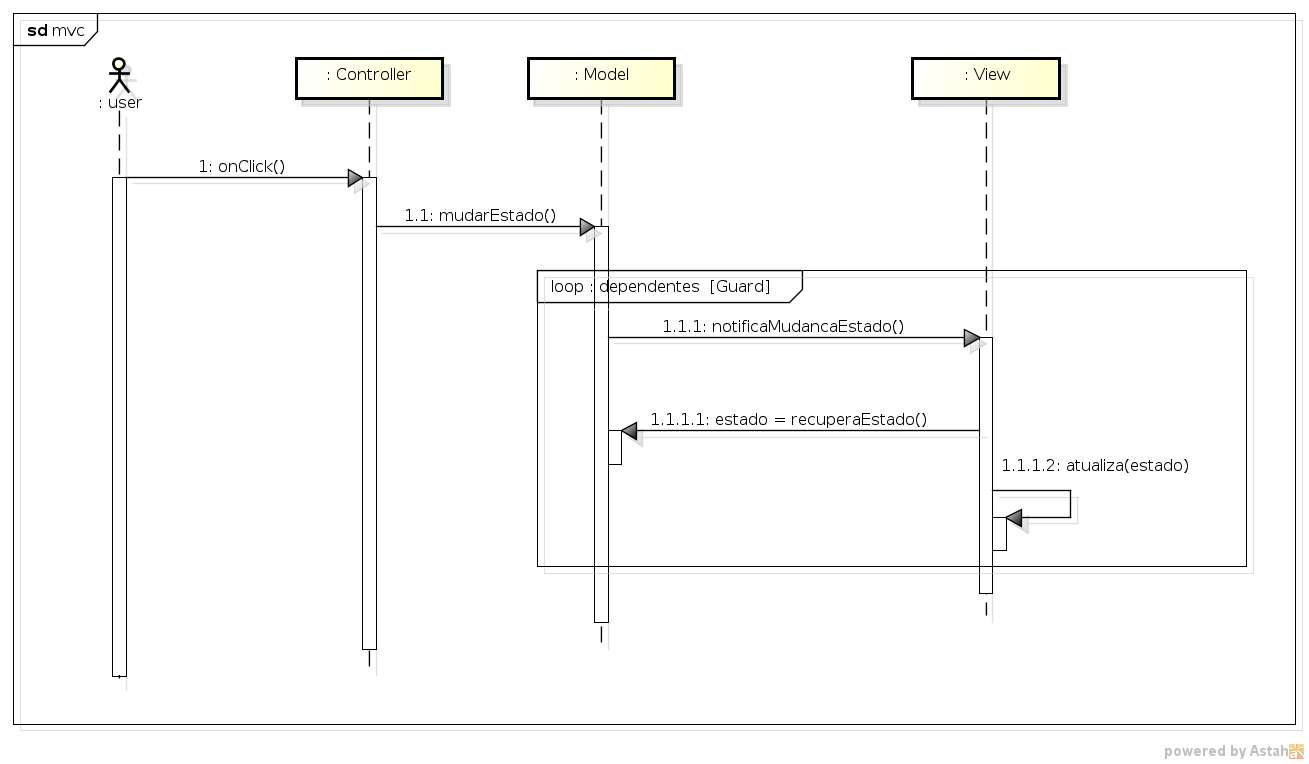
\includegraphics[scale=0.5]{img/mvc_seq.png}
	\caption{Diagrama de Sequência do MVC/Fonte: Próprio Autor}
	\label{mvc_seq}
\end{figure}

\citeonline{gof} cita \citeonline{krasnerPope1988} fazendo uma análise dos
objetos que compõem o MVC relacionando-os com outros padrões de proejto
descritos em seu catálogo.
O desacoplamento entre a View e o Model, somado à propagação das mudanças de
estado no model para os objetos regitrados como dependentes do model pode ser
descrito como uma implementação do padrão Observer. O padrão Observer define uma
estrutura em que um componente que precisa publicar mudanças em seu estado, detém a
referência para uma lista de objetos a serem notificados. A hierarquia de views
é um exemplos de Composite pois uma view pode ser constituída por sub-views para
compor views complexas. No Composite  um conjunto de componentes podem ser
tratadas de forma encapsulada onde cada implementa as mesmas abstração. O padrão
Strategy define uma abstração cuja as implementações podem ser trocadas de
acordo com algum critério, esse conceito pode ser aplicado ao controller que
encapsula o algoritmo que vai alterar a View e o Model, permitindo sua
substituíção por uma outra implementação que deixa de responder às interações
com o usuário.

Segundo \citeonline{krasnerPope1988} o Model ``\ldots pode ser simples como
um valor numério inteiro (como o modelo de um contador) ou um valor literal
(como o modelo de um editor de texto), ou pode ser um objeto
complexo''(tradução livre).
O model pode ser implementado usando o pardrão Facade para simplificar as
interações com o Model dependendo da complexidade do domínio que ele
representa.

\section{Model View Presenter}

O MVP é um modelo de programação para implementação de interfaces com o usuário
desenvolvido como um framework para C++ e Java, criado por uma subsidiária da
IBM chamda Taligent,Inc. Este padrão é baseado no MVC e descreve vários componentes que tem as
responsabilidades de como gerenciar os dados da aplicação e como o usuário
interage com esses dados, tendo como objetivo promover o encapsulamento do Model
, reuso de lógica de negócio e o polimorfismo da View.

\begin{description}
  \item[Model] Tem as mesmas responsabilidades que o Model definido pelo MVC.
  \item[Selections] - Abstração para selecionar um subconjunto dos dados
  existentes no model.
  \item [Commands] Representa as operações a serem executadas sobre uma
  Selection do Model.
  \item [View] Responsável por exibir o model assim como no MVC.
  \item [Interactor] Mapeia os interações do usuário na view como eventos do
  mouse.
  \item [Presenter] O papel do presenter é interpretar o eventos iniciados pelo
  usuário executando a lógica de negócio correspondente implementada em um
  command para manipular o model \cite{Potel96mvp}.
\end{description}


Os conceitos do MVP são descritos em \citeonline{Potel96mvp} de forma genérica
permintindo interpretações para uma implementação efetiva.
\citeonline{twisttriad:2000} descreve a implementação de um framework para
Dolphin Smalltalk\footnote{Implementação da Linguagem de programação Smalltalk - 
\url{http://www.object-arts.com}} adotando os conceitos do MVP onde salienta que
a maioria dos sistemas operacionais com ambiente gráfico fornece um conjunto de
componentes (Widgets) no qual está contido a responsabilidade do controller.A
maior parte do comportamento do caso com o usuário é implementada no
Presenter que está diretamente associado à View.

Ainda acerca das responsabilidades do Presenter, \citeonline{fowler:ui} descreve
o que é chamado de Passive View, onde toda a lógica do comportamento da view é
implementado no presenter deixando a view enxuta com o intuito de isolar ao
máximo a API gráfica do resto da aplicação. Dessa forma o model não se comunica
com a view por meio do observer pattern, sendo que a view séra atualizada pelo
presenter como pode ser observado na Figura~\ref{fig:mvp_passive_view}.

\begin{figure}[h]
	\centering
	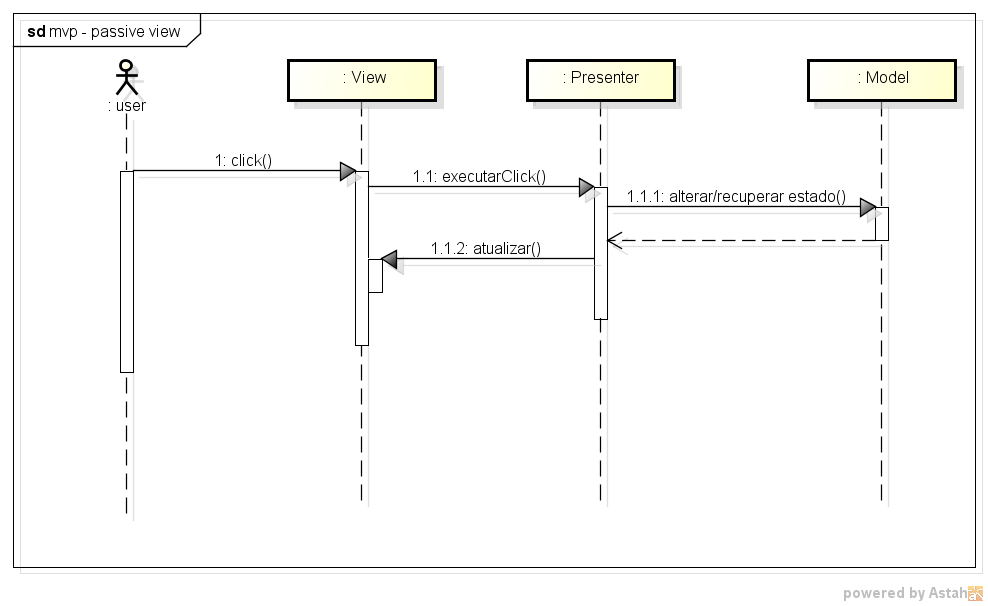
\includegraphics[scale=0.5]{img/mvp_passive_view.png}
	\caption{Passive View/Fonte: Próprio autor}
	\label{fig:mvp_passive_view}
\end{figure}

MVP se adequa melhor as apis gráficas existentes e define de forma mais clara os
componetes necessários para desenvolver uma aplicação, sendo o ponto de maior
discussão reside em quais os limites das responsabilidades no que tange a
mediação do Model e a View por parte do Presenter.

\section{Framework Android}
 

O android é um sistema operacional baseado no linux mantido pela Google para
ser embarcado em dispositivos podendo ser aplicado em carros, televisão, placas
controladoras mas seu destaque é a utilização em smartphones e
tablets, que é o foco deste trabalho. A plataforma é contituída por API's e
frameworks tendo em sua base o sistema operacional e seus drivers seguido da
máquina virtual que executa os aplicativos android e bibliotecas auxiliares e
aplicativos básicos como é demonstrado na figura \ref{android_stack}.

\begin{figure}[h]
	\centering
	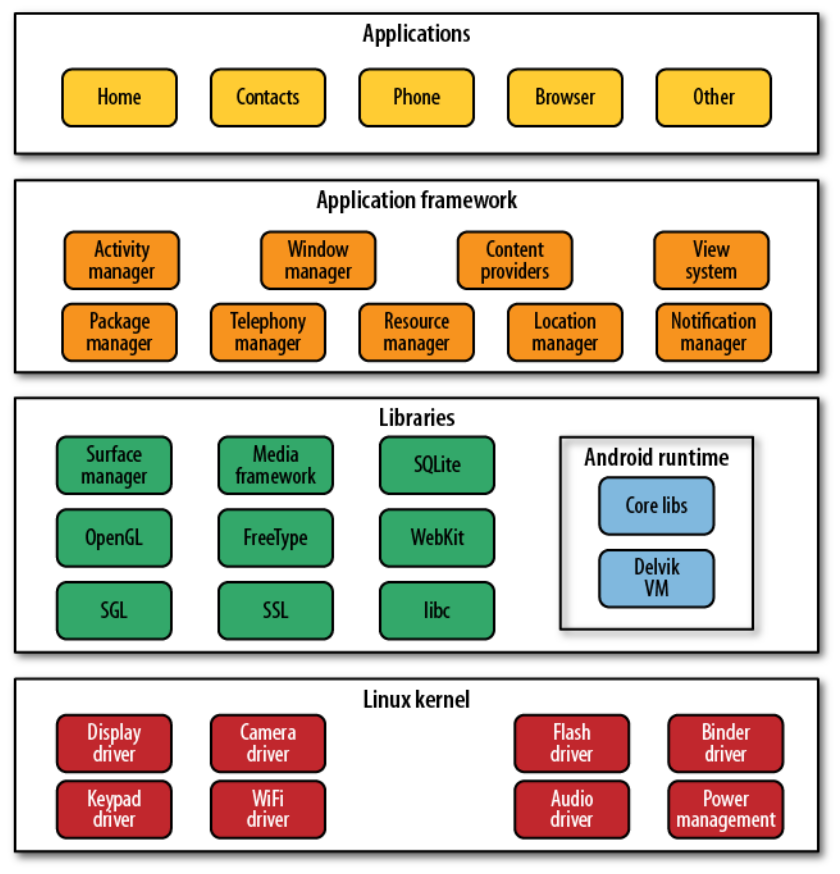
\includegraphics[scale=0.5]{img/android_stack.png}
	\caption{Android Stack/Fonte: Learning Android}
	\label{android_stack}
\end{figure}

Para desenvolvimento é usado a api disponível no sdk que define
os blocos de construção de um aplicativo, a saber:

\begin{description}
  \item[Activity] Representa uma atividade que o usuário executa no aplicativo
  em um determinado momento. É um agregador de componetes visuais e responde à
  interações do usuário.
  \item[Fragment] Representa uma parte de interface com o usuário em uma
  Activity.
  \item[Service] Responsável por executar uma operação sem interface gráfica
  indicado para processamentos longos como por exemplo a execução de uma música
  ou download de de arquivos.
  \item[Broadcast Receiver] Implementação do padrão publish/subscribe 
  \item[Content Provider] Usado para expor dados de uma aplicativo para outros
  aplicativos. Os dados podem ser provenientes de qualquer forma de
  armazenamento como um arquivo ou banco de dados.
  \item[ApplicationContext] Representa a aplicação em execução provendo acesso
  a recursos.
  \item[AsyncTask] Usado para implementar computação paralela evitando o uso da
  linha de execução principal do aplicativo que é respoonsável por tratar a
  interações com o usuário.
\end{description}

Com base nos componentes de framework e literatura revisada é possível fazer
uma análise dos mesmos e projetar uma camada de apresentação utilizando o padrão
MVP para ser usada como referência de implementação a ser aplicada.


\section{Refatoração do Objeto de estudo}

Com base na literatura revisada esta seção tem como objetivo fazer uma análise
dos componentes do framework android e projetar uma camada de apresentação
utilizando o padrão MVP. Será realizado uma análise  tendo como objetivo definir
usada um referência de implemntação a ser aplicada na refatoração(Referências
sobre Refatoração de Código)
Quem vai ser o model?

\begin{center}
\begin{tabular}{ | l | l | l | }
  \hline                        
  	Model & View & Presenter \\  \hline
  	Dao & Activity & POJO \\  \hline
\end{tabular}
\end{center}

OnTouchListener pode exercer papel de controller pois
pode ser usado para interpretar os gestos do usuário e direcioar para o model.


%Explicar uso do padrão observer no mvc
Na definição clássica do padrão MVC é possível identificar a implementação do
padrão Observer usado para a comunicação entre o model e a view.

Observer=Lapsed listener problem=memory leak e bugs porque uma activity pode ser
ou estar sendo referenciada por um listener que se não for desregistrado vai
causar problema

Destacar problema com o observer pattern e pra solucionar isso
usar publish–subscribe messaging pattern

O Broadcast Receiver é uma implementação do padrão pubsub onde diversos
subscribers se registram para receber mensagens(intents) de seu interesse.


Padrões Criacionais. O objeto Application é um singleton, a activity e
fragmentos são criados pelo android e fica dificil aplicar padrões criacionais é
possível identificar o padrão templete method nos ciclos de vida desses
componentes.



 Para concluir a seção sobre MVC e MVP destacar que A principal características
 desses padrões de projetos é que ele promover maior coesão nos citar Tom deMarco 

baseado em outras pesquisa será aplicado padões de projetos  para melhorar a
 qualidade pegar referências,  relacionar Coesão = Qualidade.

\chapter{Resultados e Conclusões}



\section{Trabalhos Futuros}

Existem outros padrões de projetos para o desenvolvimento da camada de
apresentação de um software que não foram analisados nesse trabalho: MVVM,
MVP-VM, MVPC.

Este trabalho não fez uma avaliação dos impactos na performance do aplicativo
devido ao uso desses padrões. A inclusão de mais objetos interagindo,
redirecionando mensagens pode depreciar a performance.


\section{Conclusões}

Validade dessas métricas, talvez o ideal fosse customizar essas métricas para o
framework.
Possível aumento do código.


% ---
% Finaliza a parte no bookmark do PDF, para que se inicie o bookmark na raiz
% ---
\bookmarksetup{startatroot}% 

% ----------------------------------------------------------
% ELEMENTOS PÓS-TEXTUAIS
% ----------------------------------------------------------
\postextual


% ----------------------------------------------------------
% Referências bibliográficas
% ----------------------------------------------------------
\bibliography{abntex2-modelo-references}

% ----------------------------------------------------------
% Glossário
% ----------------------------------------------------------
%
% Consulte o manual da classe abntex2 para orientações sobre o glossário.
%
%\glossary


\end{document}
